\usepackage{pgf}
\usepackage{tikz}
\usetikzlibrary{arrows,automata,plotmarks}
\usepackage{pgfplots}
\pgfplotsset{compat=1.15}

\tikzset{
    % node styles
    state-node/.style={
        fill=none, shape=circle, draw=black, thick, text=black, minimum size=0.6cm},
    action-node/.style={
        fill=black, draw=none, text=white, shape=circle, inner sep=0.05cm, minimum size=0.2cm},
    reward-node/.style={
        fill=none, draw=black, text=black},
    hidden-node/.style={
        fill=none, draw=none, text=white, shape=circle, inner sep=0,outer sep=0, minimum size=0.0cm},
    % label styles
    action-label/.style={
        shape=circle, text=white, draw=none, fill=black, inner sep=0.05cm, minimum size=0.2cm, align=center, yshift=0.0cm, anchor=center},
    reward-label/.style={
        shape=rectangle, text=black, draw=black, fill=white, minimum size=0.5cm, align=center, yshift=0.0cm, anchor=center},
    hidden-edge/.style={
        text=white, draw=none, fill=none, inner sep=0,outer sep=0, minimum size=0.0cm},
}


% Diagrama de interação
\newcommand{\rlinteraction}{
    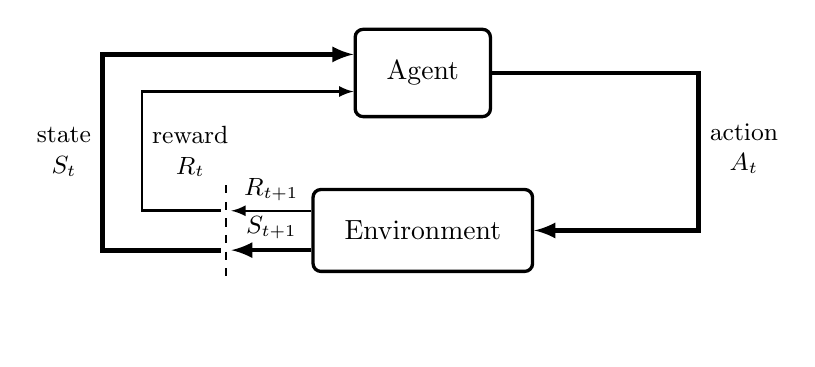
\begin{tikzpicture}[->,>=latex, auto, node distance=2.0cm, very thick, font=\small]
        \tikzstyle{rect-node}=[fill=none,shape=rectangle,draw=black,text=black,rounded corners=0.1cm, inner sep=0.4cm]
        \tikzstyle{hidden-node}=[fill=none, draw=none, text=black, shape=rectangle, inner sep=0,outer sep=0.05cm, minimum height=0.75cm]
        
        \node[rect-node]  (Agent)                                     {\normalsize Agent};
        \node[rect-node]  (Env)     [below of=Agent]                  {\normalsize Environment};
        \node[hidden-node] (Hidden)  [left of=Env, xshift=-0.5cm]     {};
        \node[hidden-node] (UpHid)   [above of=Hidden, yshift=-1.0cm] {};
        \node[hidden-node] (DownHid) [below of=Hidden, yshift=1.0cm]  {};
        
        \draw[thick, transform canvas={yshift=0.25cm}] (Env) to node[above] 
            {$R_{t+1}$} (Hidden);
        \draw[ultra thick, transform canvas={yshift=-0.25cm}] (Env) to node[above] 
            {$S_{t+1}$} (Hidden);
        \draw[ultra thick] (Hidden.255) to node[left, pos=1.0, yshift=1.25cm, align=center] 
            {state\\$S_t$}  ++(-1.5,0) |- (Agent.165);
        \draw[thick] (Hidden.105) to node[right, pos=1.0, yshift=0.75cm, align=center] 
            {reward\\$R_t$} ++(-1.0,0) |- (Agent.195);
        \draw[ultra thick] (Agent) to node[below right, pos=1.0, yshift=-0.5cm, align=center] 
            {action\\$A_t$} ++(3.5,0)  |- (Env);
        \draw[-, thick, dashed] (UpHid) to node {} (DownHid);
    \end{tikzpicture}
}